


\section{Tsetlin Machine Fundamentals}
\label{sec:tmtheory}
The Tsetlin Machine (TM) is a learning algorithm based on propositional logic and finite-state automata. It represents patterns using Boolean formulas, with its structure defined by clauses, whose composition is controlled by collections of Tsetlin Automatas (TAs). This section will take a closer look at the core components of the TM: literals, clauses, learning automata and the principles of training and inference.

\subsection{Features and literals}
In machine learning, a feature is a measurable property or characteristic of the input data. Features provide the information a model needs to distinguish between classes or to make a prediction. For example, in a simple classification task distinguishing between apples and oranges, features might describe color, shape, or texture. Each feature $x_i$ captures one aspect of the data, and together they form a feature vector
\begin{equation}
\label{eq:featvec}
    X = [x_0,x_1,...,x_{o-1}].
\end{equation}

As mentioned earlier, one of the qualities contrasting the TM from other learning algorithms is that it operates on Boolean features, meaning each feature is either \textit{True} or \textit{False}. In the apples and oranges task, the features might be:

\begin{itemize}
    \item $x_0$ = 1: sphere-shaped
    \item $x_1$ = 1: orange color
    \item $x_2$ = 1: smooth skin
\end{itemize}

Some features may apply to multiple classes, for example both apples and oranges are \textit{roughly} sphere-shaped, while others might be more exclusive (i.e. orange color).

In addition to the standard features, the TM appends the feature vector $X$ with the negated features $\neg x_i$. Together, the features and their negated self are called \textit{literals}, and a literal represents either the presence or absence of a characteristic. The new input vector containing literals is called $L$. Note that the input vector length has now grown from $o$ to $2o$.

\begin{align}
\label{eq:literalvec}
    L &= [l_0, l_1, ..., l_{2o-1}] \\
      &= [x_0, ..., x_{o-1}, \neg x_0, ... \neg x_{o-1}]
\end{align}

Literals form the basic components of logical expressions learned by the TM. Since literals are Boolean, their evaluation can be reduced to simple bitwise operations. The next section introduces clauses, which combine literals into interpretable logical patterns.

\subsection{Clauses}
\label{sec:clauses}
A clause is a propositional expression which is formed as a conjuction (logical AND) of literals. A clause $C_j$ over a set of literals $L$ can be written as 

\begin{equation}
\label{eq:clause}
    C_j = \bigwedge\limits_{l_k \in S_j} l_k,
\end{equation}

where $S_j$ is the subset of literals chosen to belong to the clause. Literals not included in $S_j$ therefore do not influence the clause's output. Returning to the apples or oranges example, a set of clauses might look like this:

\begin{itemize}
    \item $C_0 = \neg x_1 \wedge x_2$
    \item $C_1 = x_1$
\end{itemize}

These clauses can be translated to interpretable descriptions, with $C_0$ meaning ''not orange-colored AND smooth-skinned'', indicating apple, and $C_1$ meaning ''orange-colored'', which might be sufficient to classify an orange.

In binary classification, clauses are typically divided into positive and negative clauses, with positive clauses voting \textit{for} the target class, and negative clauses voting \textit{against} the target class. The final class score is obtained by summing clause outputs. This voting scheme allows the TM to combine multiple clauses capture wider range of patterns and characteristics of each class.

\subsection{Tsetlin Automata}

Tsetlin Automata are simple finite-state machines first introduced by Mikhail Tsetlin in 1961 \cite{Tsetlin1961}. They are one of the central components of TMs, tasked with determining wether a literal should be included in a clause or not. Each literal in each clause is assigned its own automaton, meaning the TM contains many TAs working in parallel.
\begin{figure}[H]
    \centering
    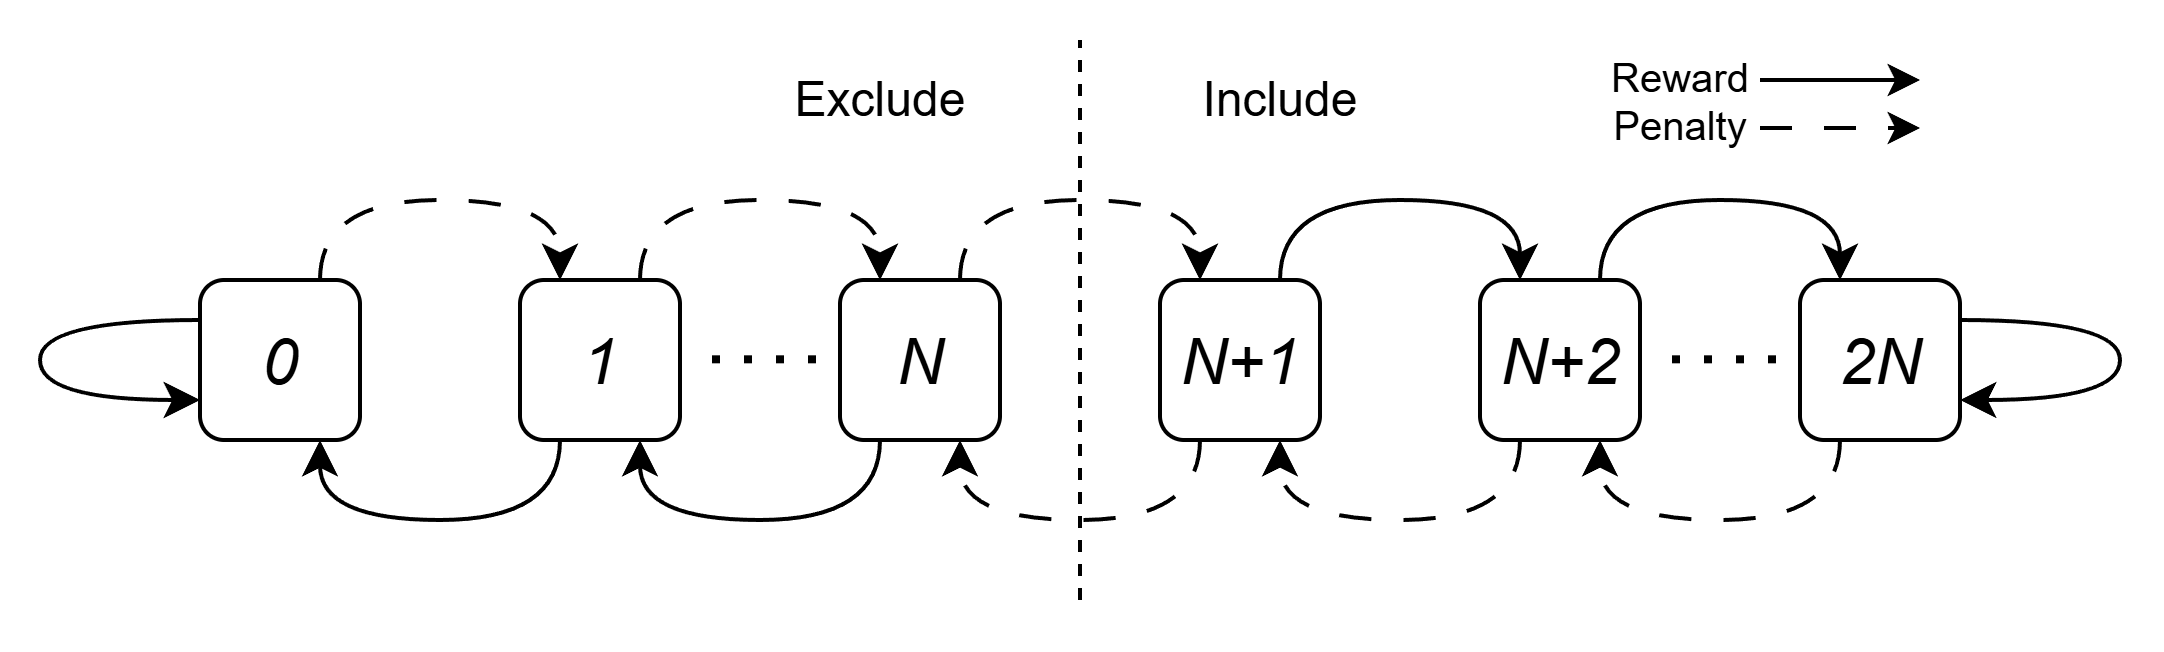
\includegraphics[width =1.1 \textwidth]{Figures/TsetlinAutomata.png}
    \caption{State diagram of a Tsetlin Automaton.}
    \label{fig:tsetlinautomata}
\end{figure}
To decide wether to include or exclude a literal, a TA maintains an internal state, as shown in Figure \ref{fig:tsetlinautomata}. The states are divided into two halves, with the first half corresponding to Exclude, and the second half corresponding to Include. The state of the TA is updated during training by feedback received from the TM. In short, the TA either receives a Reward, strengthening its decision and moving the state deeper into the current half, or a Penalty, encouraging change by moving the state toward the opposite half. Through repeated TA state updates, the automata gradually learns which literal are relevant to describing a given class.

Going back to the apples and oranges example, a TA responsible for $x_1$ (orange color) might learn to include it in a clause detecting oranges, while TAs for $x_0$ (sphere-shaped) might learn to exclude it as it might not provide meaningful insight to distinguish the two fruits. Each TA operates independently, but together they shape the clauses into meaningful patterns.

This simple state-based mechanism allows the TM to update clauses using lightweight, interpretable rules. The next section describes how TAs interact with clause outputs during training, and how the TM uses the resulting patterns during inference.

\subsection{Training and inference}

Training in the Tsetlin Machine revolves around adjusting the composition of clauses by updating the states of the Tsetlin Automata described in the previous section. During training, the TM evaluates how well each clause contributes to correct classification and generates feedback that guides the automata toward more useful literal selections. This feedback is typically divided into two types: Type I and Type II, which respectively promote true positive patterns and suppress false positives. A comprehensive explanation of these mechanisms can be found in the foundational TM literature \cite{GranmoOle-Christoffer2018TTM-}.

In essence, training iteratively refines each clause so that it captures patterns characteristic of a target class. As the automata update their states based on rewards and penalties, the TM gradually forms a set of Boolean expressions that together describe the structure of the data.

Inference, by contrast, is straightforward and computationally lightweight. Given an input sample, each clause evaluates to either 1 or 0 depending on whether all of its included literals are satisfied. Clauses are typically divided into positive and negative groups, voting for or against a given class. The votes from all clauses are summed to produce a class score, and the class with the highest score is selected as the prediction. Figure \ref{fig:tmblock} shows a high-level view of the inference structure for a multi-class TM, note the added argmax block used to decide which class has the highest score.

\begin{figure}[H]
    \centering
    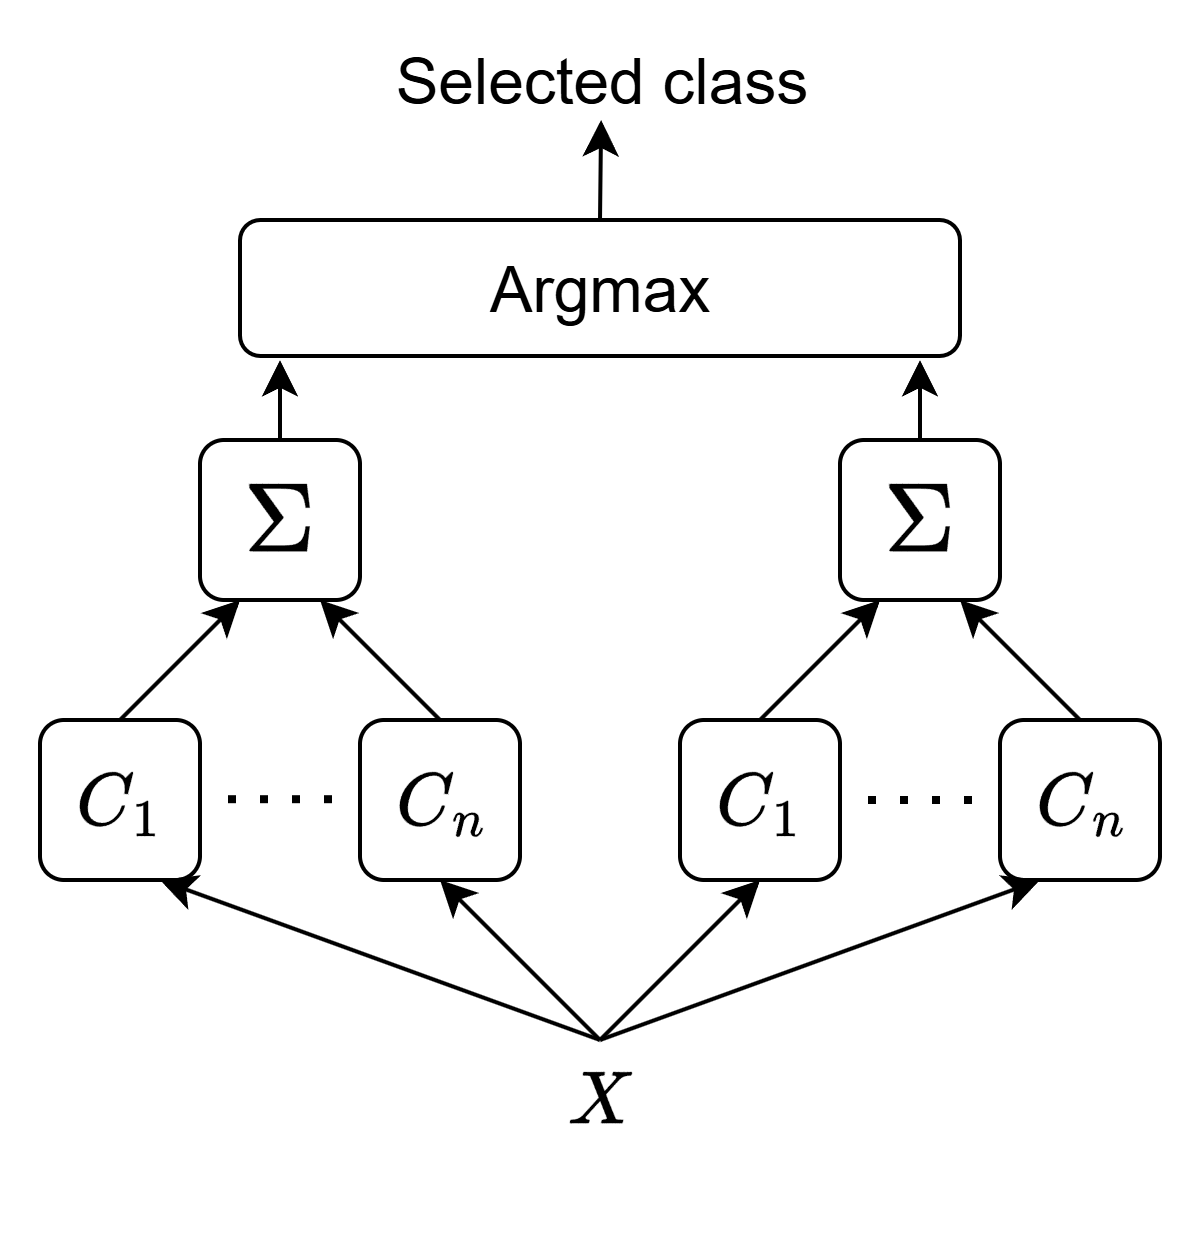
\includegraphics[width =0.6 \textwidth]{Figures/mctm_blokk.png}
    \caption{Block diagram of multi-class Tsetlin Machine.}
    \label{fig:tmblock}
\end{figure}

Because clause evaluation consists solely of Boolean operation, checking literals and combining results with logical AND, and inference requires no state updates, the inference phase is particularly well suited for hardware acceleration. This project focuses on exploiting this property by designing custom processor extensions that speed up clause evaluation and class scoring.
